\PassOptionsToPackage{table}{xcolor}
\documentclass[11pt,oneside,draft]{amsart}	%defines this as an article
\usepackage{chrisfriend-comp} %provides formatting declarations for page, headers, figures, textcolor, comments, and bibliographic styles
\usepackage{chrisfriend-OTF-support} %provides support for OTF system fonts; incompatible with latex, rtf2latex, & ht4latex
%\usepackage[utf8]{inputenc} %support for smallamp?

%\usepackage{tabularx}
\usepackage{tabulary} % allows for the tables I make rubrics with
%\usepackage{supertabular}
\usepackage{xtab} % allows tables to span pages
\usepackage{booktabs} % allows fancy lines in tables
%\usepackage{rotating} % allows landscape tables
\usepackage{lscape} % allows rotated longtables
\usepackage{multirow} % allows rowspanning
%\usepackage[table]{xcolor}    % loads also »colortbl«; allows for shaded rows
\usepackage{enumitem} % helps with the overview
%\usepackage{paralist}
%\usepackage{draftwatermark}

\usepackage{acronym}
\acrodef{ucf}[\textsc{ucf}]{the University of Central Florida}
\acrodef{dwr}[\textsc{dwr}]{the Department of Writing and Rhetoric}
\acrodef{waw}[\textsc{waw}]{Writing About Writing}
\acrodef{uwc}[\textsc{uwc}]{University Writing Center}
\acrodef{1102}[\textsc{enc~1102}]{Composition II}
\acrodef{rr}[\textsc{rr}]{Reading Response}


\title[\textsc{enc}~1102 Syllabus]{Course Syllabus: Composition II}
\chead{\scriptsize{\fontspec[Numbers=Lining]{Garamond Premier Pro}\MakeUppercase{ENC~1102 Syllabus}}}

  
\begin{document}
%\bibliographystyle{abbrv}
\thispagestyle{empty}
\vspace{-2in}
\begin{center}
\huge
\includegraphics[scale=.4]{pegasus.pdf}

\textbf{Course Syllabus: Composition II}
\end{center}


\label{sec:about_the_course}
\vspace{1.5\baselineskip}
\begin{center}
\begin{minipage}{0.66\textwidth}
%	|\hfill|
	\begin{description}[align=right, labelwidth=*, labelindent=0.9in, leftmargin=1in]
%	\item[Course Title] Composition II
	\item[Prerequisite] Successful completion of \textsc{enc} 1101 or a passing score on an AP English Exam
	\item[Meeting]  Online (\textsc{enc 1102.bw65})
	\item[Term] Summer B 2013
	\vspace{0.5\baselineskip} \hrule \vspace{0.5\baselineskip}
	\item[Instructor] Christopher R. Friend
	\item[Email] \href{mailto:friend@ucf.edu}{friend@ucf.edu}
	\item[Office] Colbourn Hall (\textsc{cnh}) 304\textsc{b}
	\item[Office Hours] In person or online, with appointment. \\ Visit \href{http://friend.lattiss.com}{http://friend.lattiss.com} for available times or \href{mailto:friend@ucf.edu}{email instructor} for other options.
\end{description}
\end{minipage}
\end{center}
\vspace{0.75\baselineskip}

\section{Overview} % (fold)
\subsection{Course Description} % (fold)
\label{sub:course_description}
In this course, we will explore the research process as one of genuine inquiry. During the semester, you will be expected to:
\begin{itemize}
	\item ask challenging, open-ended questions requiring inquiry to answer;
	\item read carefully what others have said about those questions; 
	\item create new knowledge about those questions using appropriate primary and secondary research methods, including library research, historical analysis, rhetorical analysis, survey, or interview; and
	\item join the existing research ``conversation'' on relevant topics.
\end{itemize}
You will use writing as a tool to help you learn each of the concepts listed above, and you will become more aware of your style and abilities as a researcher.
% subsubsection my_version (end)
% subsection course_description (end)


% section about_the_course (end)
\subsection{Course Outcomes}\label{outcomes}
Through successful completion of this course and its activities, you should be able to
\begin{itemize}
	\item read, analyze, and respond to difficult texts;
	\item understand texts as claims and test those claims;
	\item ask meaningful questions about the literacies required in the 21st century;
	\item use research and analysis to seek answers to those questions;
	\item gather and analyze data of various kinds;
	\item use technologies to help achieve writing and research goals;
	\item convey written ideas and research findings effectively for various audiences and purposes; and
	\item explain writing-related concepts, including \emph{intertextuality}, \emph{genre}, \emph{originality}, \emph{plagiarism}, and \emph{the technologies of writing and research}.
\end{itemize}


\section{Materials for Class}
\begin{enumerate}
	\item Required
	\begin{itemize}
		%\item \citeauthor{greene:2008aa}, \citetitle{greene:2008aa}\\ (\textsc{isbn} \href{http://www.worldcat.org/search?q=978-0-312-60140-9}{978-0-312-60140-9}) %(Bring to class each day.)
		%\item \citeauthor{lunsford:2010aa}, \citetitle{lunsford:2010aa}, \emph{Fourth Edition}\\ (\textsc{isbn} \href{http://www.worldcat.org/search?q=978-0-312-66486-2}{978-0-312-66486-2})%(Bring only when requested.)
		\item Reliable connection to the Internet. Make a plan for where you will go if your device or connection dies.
		\item Automated, reliable backup system. Every semester, I have a student who loses everything due to a hard drive failure. Don't be that student.
		\item Regular access to your Knights Mail account. I check my account multiple times per day. You need to check yours \emph{at least} once per day, but preferably more frequently.
	\end{itemize}
	\item Recommended
	\begin{itemize}
		\item Google account connected to your Webcourses (Canvas) account. This helps make collaboration a breeze.
		\item Dropbox account into which you store all your work. This takes care of backups.
		\item Your own computer running a full (non-mobile) operating system. Some of the work we do is much simpler if you can install new software and run multiple programs simultaneously. Phones are too limited, and iPads get frustrating\footnote{Various computer labs across campus, or the loaner machines at the library, can work in a pinch.}.
	\end{itemize}
\end{enumerate}

\section{Grading \& Assessment}
Your grade in this course will be based on two holistic grades listed in Figure~\ref{tab:assignments}. Think of these like grades for a semester-long portfolio: the components work together to build the overall value of the whole. That value is what will be graded in this course. You will get consistent feedback throughout the semester to help ensure you are on-track for a successful grade. Additionally, each major assignment will have a specific assessment rubric, and every smaller assignment will have detailed completion guidelines that will be provided in class and available on Webcourses.  The smaller assignments are designed to help you build skills and confidence as you work toward your final project. They should not be dismissed.

Please note the following distinctive characteristics about grading in this course:
\begin{itemize}
	\item You can earn a D for an assignment or major component, but you cannot earn a D for this course. To pass, you must earn at least a C average.
	\item The grade of NC (no credit) can be assigned at the instructor’s discretion only if you complete all course work on time, attended class regularly, and fail to produce satisfactory work for the class.
\end{itemize}


\subsection{Grading Standards} % (fold)
\label{sub:grading_standards}
Participation in all activities, and successful completion of all assignments (as defined by each assignment's assessment rubric) will earn you a passing grade of C, indicating that you have achieved the expected outcomes of the course. If you do not take part in all assignments and activities, you should not expect a passing grade in the course. If the quality of your work or your participation falls below acceptable standards (i.e. if you are heading for failure), I will be sure to let you know. Along more optimistic lines, grades of B or A are used for work that is good and excellent, respectively, surpassing the basic expectations. Assignment sheets will suggest ways to exceed those expectations, so you won't have to guess. If your performance exceeds basic standards, I will be sure to let you know.

Besides participation, all grades for this course come from products turned in at the end of the semester (see Figure~\ref{tab:assignments}). This is by design, to allow you the chance to experiment and take risks as you progress through the course. If your research leads you down a dead-end, your grade will not be affected. In lieu of grades, you will receive constant feedback from your peers and instructor about what is and isn't working well with your research and various written products. Take the feedback seriously, and revise your work regularly throughout the semester so that your final portfolio best reflects your ability.

Please note these odd characteristics of grading in this course:
\begin{enumerate}
	\item You will not earn a grade on any assignment before the final portfolio. You'll get feedback, but not a grade.
	\item \textbf{You cannot pass this course unless you earn a passing score on the portfolio.} In other words, a passing score (≥60 points) on your portfolio qualifies you to have your portfolio and participation scores averaged into a final grade.
\end{enumerate}
% subsection grading_standards (end)

\begin{figure}[t] 
	\centering
	\subtable[Grade Calculations]{\small
		\noindent\begin{tabulary}{0.25\textwidth}{lr}
		\toprule\textbf{\textsc{Grade}} & \textbf{\textsc{Min. Points}}\\
		\midrule
			A	&	185	\\
			A-	&	180	\\
			B+	&	175	\\
			B	&	165	\\
			B-	&	160	\\
			C+	&	155	\\
			C	&	145	\\
			C-	&	140	\\
			NC	&	Unsatisfactory	\\
			F	&	Partial/Poor	\\
		\bottomrule
		\end{tabulary}\label{tab:final-grades}
	} %subtable
	\quad % Middle gap spacing
	\subtable[Grade Distribution]{\small
		\noindent\begin{tabulary}{\textwidth}{Lr}
			\toprule\textbf{\textsc{Assignment}} & \textbf{\textsc{Points}}\\
				\midrule	Products (portfolio w/ papers and course audit)	&	100	\\
%				\midrule	Academic Research Report	&	25	\\
%				\midrule	Genre Product \& Presentation	&	25	\\
				\midrule	Process (participation \& collaboration)	&	100	\\
				\midrule	\textbf{\textsc{Total}}	& \textbf{\textsc{200}}\\
			\bottomrule
		\end{tabulary}\label{tab:assignments}
	} %subtable
	\caption{Course Grading System}
\end{figure}


\subsection{Expectations} % (fold)
\label{sub:expectations}
This class will employ collaboration to a larger extent than is perhaps typical in a composition course. You will not be doing group projects, but you will be working with one another to learn from one another's work, progress, and feedback.

While enrolled in this course, you can expect these things from me:\footnote{The structure and approach of the Expectations section is adapted from the \href{http://www.ceball.com/classes/239/spring09/?page_id=8}{English 239 syllabus} of Cheryl E. Ball, \textsc{isu}.}
\begin{itemize}
	\item enthusiasm for research, teaching, and writing;
	\item clarity and thoroughness in assignments, goals, and expectations;
	\item personal interest in your learning and work;
	\item freedom to be creative with the products you create for this course;
	\item critical feedback to help you improve your thinking and writing; and
	\item preparation to ensure a beneficial and productive semester.
\end{itemize}
If at any point you feel I am failing to meet any of those expectations, please let me know. Your feedback is the best way I can learn how to improve my teaching.

As we progress through the semester, your peers and I will expect these things from you:
\begin{itemize}
	\item consistent and active participation in class activities, including peer review assignments;
	\item informed contributions, based on sufficient preparation and consideration (i.e. doing the readings and research)
	\item an open mind, tolerant and curious about differences of opinion; and
	\item honest and polite commentary and feedback that helps your peers improve their work.
\end{itemize}

During class discussions and as you work on your assignments, keep in mind that I value these things in my students:
\begin{itemize}
	\item thought-out and supported opinions;
	\item willingness to take risks and try new approaches to solving problems, as risks often create the greatest opportunities;
	\item creativity in how you respond to the challenges created and faced by this course; and
	\item excellence in your work, showing the best you can produce.
\end{itemize}

% subsection expectations (end)


\section{Major Assignments} % (fold)
This course builds to a final project designed to persuade people to take action on a literacy-related issue (broadly defined) of your choosing. Each unit of study (see Figure~\ref{fig:vis-syllabus}, \nameref{fig:vis-syllabus}) includes a major writing assignment designed to form, refine, and express your ideas toward that final project. For each assignment, you will receive a detailed assignment sheet with specific procedures, expectations, and an evaluation rubric. An abridged overview of each major assignment appears below.

\begin{figure}[t]
	\centering
		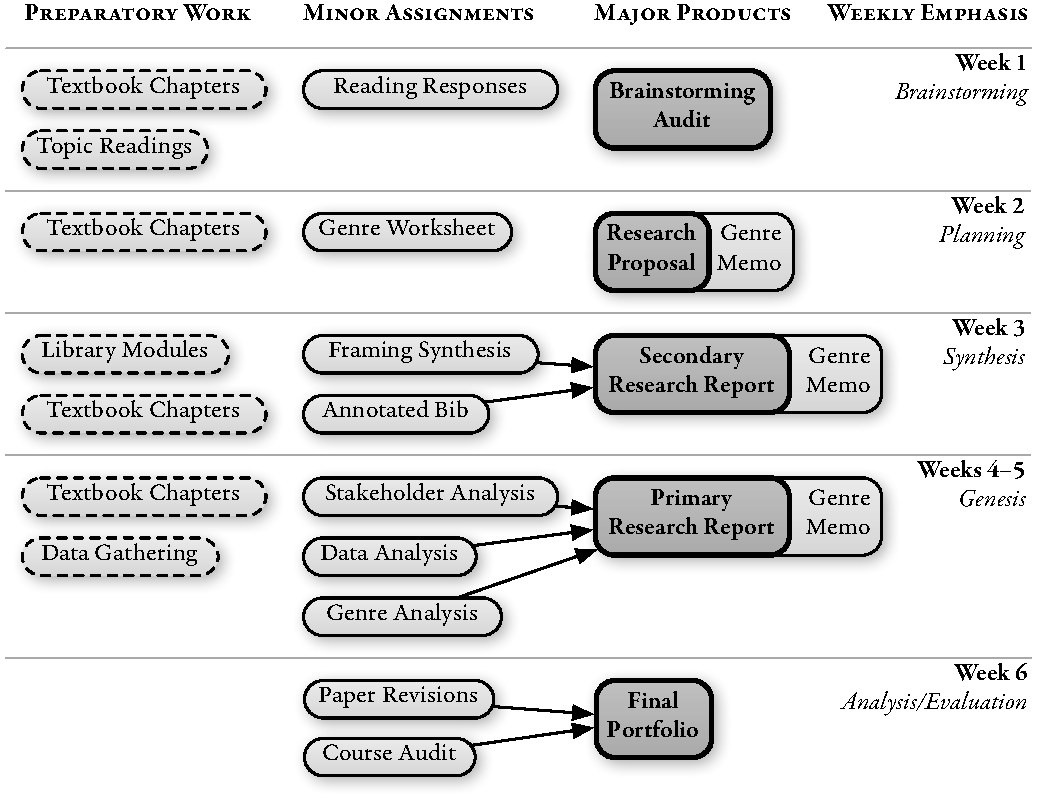
\includegraphics[width=\textwidth]{visual-syllabus.pdf}
	\caption{Course Assignments Overview}
	\label{fig:vis-syllabus}
\end{figure}


\subsection{Brainstorming Audit} % (fold)
\label{sub:brainstorming_reflection}
	\begin{description}
	\item[Task] Choose a potential issue or question you would like to research, based on the readings at the beginning of the semester. Document your decision and what led you to it.
	\item[Purpose] Show that you can:
		\begin{enumerate}
		\item identify a relevant, researchable problem;
%		\item determine and explain why you are interested in that problem;
		\item specify what you wish to learn about the problem; and
		\item document and properly cite the readings that led to your decision.
		\end{enumerate}
	\end{description}
% subsection brainstorming_reflection (end)

\subsection{Research Proposal} % (fold)
\label{sub:research_proposal}
	\begin{description}
	\item[Task] Create a plan for conducting a semester-long research study.
	\item[Purpose] Show that you can:
		\begin{enumerate}
		\item identify a clear research problem or question,
		\item create a plan of action for exploring your chosen issue,
		\item show that your study is important and relevant, and
		\item suggest a target audience for your findings.
		\end{enumerate}
	\end{description}
% subsection research_proposal (end)

\subsection{Secondary Research Report} % (fold)
\label{sub:context_analysis}
This assignment has two components that combine to document the situation and existing knowledge in which your research is taking place.
\subsubsection{Annotated Bibliography} % (fold)
\label{ssub:annotated_bibliography}
	\begin{description}
	\item[Task] Create a list of sources related to the issue you are investigating.
	\item[Purpose] Show that you can:
		\begin{enumerate}
		\item identify a variety of sources related to your issue,
		\item describe other people's research methods and claims, and
		\item evaluate the validity of claims and arguments.
		\end{enumerate}
	\end{description}
% subsubsection annotated_bibliography (end)
\subsubsection{Framing Synthesis} % (fold)
\label{ssub:framing_synthesis}
	\begin{description}
	\item[Task] Present your collection of sources as a cohesive whole.
	\item[Purpose] Show that you can:
		\begin{enumerate}
		\item explain the relationships among sources,
		\item relate your sources to the question or problem you are researching,
		\item identify the shape and nature of present conversation around the issue.
		\end{enumerate}
	\end{description}
% subsubsection framing_synthesis (end)
% subsection context_analysis (end)

\subsection{Primary Research Report} % (fold)
\label{sub:outcomes_analysis}
This assignment has three components that combine to move the existing knowledge on a topic forward, growing from the positions identified in the Secondary Research Report.
	\begin{description}
	\item[Task] Create knowledge about your chosen issue; determine how that information would best be used.
	\item[Purpose] Show that you can:
		\begin{enumerate}
			\item gather new knowledge about your chosen issue through appropriate primary research,
		\item identify the people involved in the conversation,
		\item examine their relation to the issue in a stakeholder analysis,
		\item determine what genres are used by those stakeholders, and
%		\item evaluate which genre would be most effective for your final project.
 		\item make decisions regarding your chosen issue based on the items above.
		\end{enumerate}
	\end{description}
% subsection outcomes_analysis (end)


\subsection{Final Portfolio} % (fold)
\label{sub:final_portfolio}
This assignment combines the major assignments listed above into a single document that reflects your progress through the semester. The portfolio includes a Course Audit that serves as a cover letter, reflecting on the semester and directing readers to the accomplishments seen in your work. This assignment will:
	\begin{enumerate}
	\item demonstrate how your research this semester has met the desired \nameref{outcomes} and
	\item show self-awareness of your writing and research practices.
	\end{enumerate}
% subsection final_portfolio (end)

% section major_assignments (end)




%\begin{comment} %%%%%%%%%%%%%%%%%%%%%%% Calendar


%\begin{landscape}
%\clearpage
%\addtocounter{page}{-2}
\section{Course Calendar}
\todo[inline]{Update calendar workfile; insert data here.}
%\addtocounter{page}{-1} %accommodates the blank page before Calendar
%\begin{center}
{\centering\footnotesize %brace balanced at end of calendar
%\vspace{-1in}
\tablehead{\toprule\textbf{\textsc{Unit}} & \textbf{\textsc{Week}} & \textbf{\textsc{Date}} & \textbf{\textsc{Readings/Homework}} & \textbf{\textsc{Issues for Discussion}}\\}
\tablelasthead{\toprule\textbf{\textsc{Unit}} & \textbf{\textsc{Week}} & \textbf{\textsc{Date}} & \textbf{\textsc{Readings/Homework}} & \textbf{\textsc{Issues for Discussion}}\\}
\begin{mpxtabular}{>{\bfseries}p{0.75in}ccp{1.8in}p{1.85in}} % for portrait
%\begin{xtabular}{>{\bfseries}lccp{2.25in}p{3.25in}} % for landscape
\midrule
%	\toprule\textbf{\textsc{Topic(s)}} & \textbf{\textsc{Week}} &\textbf{\textsc{Class Discussion}} & \textbf{\textsc{Readings/Homework}}\\

% Do not edit manually. Paste content in from Calendar Workfile. (Numbers document, this folder.)







 	\bottomrule
    \end{mpxtabular}
} %matches the \footnotesize at top of calendar
%    \end{center}


  
\subsection{Changes}
    Material in the preceding schedule is subject to change at the discretion of the instructor.  Students will be notified of any changes in class.  If relevant, changes will also be reflected on Webcourses.
%    \end{landscape}

\subsection{Final Exams} % (fold)
\label{sub:final_exams}
Because this class includes a portfolio that documents your progress over the semester, as well as a project you create as a result, there is no final exam as such. However, since your portfolio is the only document actually graded, it serves as a Really Big Deal™ and should be treated with as much attention as an exam. \textbf{Your final portfolio is due by 12:00 noon, EDT, on Friday, August 2.}
% subsection final_exams (end)
  


%\end{comment} %%%%%%%%%%%%%%%%%%% Calendar









\section{Policies \& Miscellanea}
%\nocite{Curtis:2009uq,Tripp:2009kx,Wardle:2010fk} %ensures the syllabi I stole from will be in the Works Consulted list

\subsection{Participation}
Because this is an online class, there is no relevant concept of ``attendance''. However, you should treat participation in class activities (including discussions, peer review assignments, etc.) as evidence of your efforts to attend to the course. I expect complete participation on all assignments from each student. We both know that the most boring classes are the ones where the instructor does all the talking. Don't let that be the case here. Speak your mind, provide your opinion, and join in the work. When in doubt, say something—it's the only way your peers and your instructor will know what's on your mind, and the only way we can compliment or correct, as needed.

\begin{comment}
	\subsection{Late Work}
	It is in your best interest to \emph{not} get behind in this class; getting caught up is quite difficult. Thus, I generally do not accept late work for credit. If you are experiencing special circumstances and would like to request an extension, speak with me \emph{well in advance} of the due date and use all the rhetorical strategies at your disposal to effectively make your case. I reserve the right to accept late work with or without penalty only as the circumstances warrant. 
\end{comment}

\begin{comment}
	\subsection{Grades}
	\todo{Update to reflect no-grading approach.}Your instructor uses a ten-point grade scale in this course. For all graded assignments, a ``C'' is average and indicates you have acceptably completed all requirements.  A grade below ``C'' indicates you have not met minimum standards.  ``B'' is an honor grade, awarded for work that is thoughtful and well-written. ``A'' work is excellent and goes beyond what is required.  A grade of ``D'' on an assignment indicates that the work partially fails to meet the standards of the assignment, whereas an ``F'' indicates overall failure to meet the expectations.
\end{comment}

\subsection{Gordon Rule} % (fold)
\label{sub:gordon_rule}
\ac{1102} is a Gordon Rule class, meaning that you will be writing at least four major assignments, and you must earn a ``C'' or better to earn credit for the course. The assignments that contribute to your final portfolio meet this Gordon Rule requirement.
% subsection gordon_rule (end)



\subsection{Etiquette}
In short, the members of this class, both the instructor and the students, are expected to behave courteously and professionally in all interactions.  Under that umbrella statement, the following general guidelines should be followed in any class here at \ac{ucf}.
	\begin{description}
	\item[Tolerance] Many of our discussions in class will be driven by opinions and based on challenging material.  Since we are all writers, everyone in class will have personal experiences and viewpoints that can contribute meaning to the conversations.  All participants are expected to treat others with dignity and respect and are expected to refrain from insensitive comments, including racist, ageist, sexist, classist, homophobic, or other disparaging and unwarranted views.
%	\item[Timeliness] Students are expected to be ready for class at its designated time just as much as you expect the instructor to dismiss class by the designated time.  Should you arrive to class late for any reason, please do so with a minimum level of disruption.  If you need to leave class early for any reason, please notify the instructor in advance and be as non-disruptive as possible when leaving.
%	\item[Cellphones] As a courtesy, all cellphones should be silenced during this or any other class. Should your phone accidentally create a distraction during class, you should take action to eliminate the distraction without adding to it.
%	\item[Computers] You will need to use your computer in class regularly to collaborate with others and complete your assignments. Having the discipline of shutting off distractions (such as Facebook, chat applications, etc.) improves your ability to focus and participate meaningfully.
	\item[Messages] Grammar, spelling, and punctuation reflect the formality of the situation in which they appear.  Keep in mind that emails and discussion posts you write for this class are being read by an English teacher in a composition course.  Though I don't expect discussion posts to be perfectly error-free (they're not that important), I do expect you to treat written language with respect. Complete sentences and full words (``you'' instead of ``u'') are always a good idea, even if the intended audience is your peers.
	\item[Email] As a \ac{ucf} student, you have access to a Knights Mail account, which will be the primary method of communication for course-related announcements and information. Because the summer semester is condensed, you should check your email at least once a day. Your instructor generally replies to messages within 24 hours Sunday through Thursday; messages sent on Fridays or Saturdays might get a delayed response.
	\end{description}
	

\subsection{Computer Reliability}\label{sub:reliability}
Save everything, and save often.  Computer problems are regular part of life, and I expect you to prepare for them rather than use them as an excuse for late work. Every semester, your instructor has students sustain a complete hard drive failure, losing all their work. Such failures are unavoidable, but losing data is not, if you plan ahead. Working backups and protection from Windows viruses are essential to avoid the most common catastrophes.  A free Dropbox account (\href{http://db.tt/mzWxY8s}{http://dropbox.com}) provides convenient and automatic backups, allows you to access your files from any networked computer in case disaster befalls yours, and preserves old versions of files so that if a file is deleted or altered, a previous copy can be restored. Regardless of the solution you choose, know how you will keep moving if your computer fails.

\subsection{Helpful Resources} % (fold)
\label{sub:helpful_resources}
\subsubsection{Writing Assistance}\label{ssub:uwc}
The \ac{uwc} provides free help for students writing papers for class.  Consultations (which can be in-person or online) can help with planning, drafting, or revising your papers.  Consider using the \ac{uwc}'s services, particularly in the early stages of planning a document.  Learn more at \href{http://uwc.ucf.edu/}{http://uwc.ucf.edu}, by calling 407-823-2197, or by visiting the first floor of Colbourn Hall.  Please note that the weeks of midterms and finals can be very busy there; you are strongly encouraged to make a reservation. A link to the \ac{uwc} appointment scheduler is available in Webcourses.

\subsubsection{Research Assistance} % (fold)
\label{ssub:knowledge_commons_in_the_library_}
Located halfway back on the main floor of the main campus library, the Knowledge Commons houses very smart, very helpful, and surprisingly friendly research assistants. They know more about the library and its collections than anyone else, and they love showing off what they know. They also don't like losing to a challenge. If you have trouble finding a particular resource or are stuck and need to find another direction to go with your thinking, they should be the first folks you talk to.
% subsubsection knowledge_commons_in_the_library_ (end)

\subsubsection{Additional Support Services} % (fold)
\label{ssub:other_support_services}
\begin{description}
	\item [Counseling and Psychological Services] 407-823-2811, \textsc{coun} 101, \href{http://caps.sdes.ucf.edu}{http://caps.sdes.ucf.edu}
	\item [Knights Helping Knights Pantry] 407-\textsc{ucf-food}, \textsc{fc-g} 171, \href{http://knightspantry.org}{http://knightspantry.org}
	\item [Student Disability Services] 407-823-2371 (TDD 407-823-2116), \textsc{fc-g} 185, \href{http://sds.sdes.ucf.edu}{http://sds.sdes.ucf.edu}
	\item [Other] See the Student Development and Enrollment Services (\textsc{sdes}) site for a complete listing of offices available to assist students:  \href{http://www.sdes.ucf.edu/departments}{http://www.sdes.ucf.edu/departments}
\end{description}
% subsubsection other_support_services (end)

% subsection helpful_resources (end)

\subsection{Plagiarism}
Students at \ac{ucf} are expected to act with integrity, in terms of both classroom behavior and intellectual property.  For details, please see the \href{http://www.goldenrule.sdes.ucf.edu}{Golden Rule Student Handbook}, section \textsc{ucf}-5.008.1.e.  Violations of this ethical cornerstone will result in disciplinary action, which can include any of the following:
\begin{itemize}
	\item loss of credit on an assignment
	\item a ``Z grade'' for the course (see \href{http://z.ucf.edu}{http://z.ucf.edu} for details)
	\item loss of credit for the course
	\item removal from the University
\end{itemize}
In an effort to protect the integrity of your work and ensure it is not re-used by others later, your instructor may ask that your assignments be submitted to Turnitin.com by their deadlines.
%\todo{Am I sure? Do I want to do this? Can it be integrated with Webcourses?}  

In this course, we will be discussing the use of outside texts for writing in and out of the classroom, specifically the use of source documentation/citation/attribution. If you have questions about correct documentation of sources, consult a writing handbook (such as \citetitle{lunsford:2010aa} by Andrea Lunsford), the style guide for the citation system you are using (such as \citetitle{gibaldi:2009aa} by Joseph Gibaldi), the \ac{uwc} (see Section~\ref{ssub:uwc}), or your instructor during office hours. Use of outside sources without proper credit, turning in work that is not your own, or assisting others to do either are each considered plagiarism and are subject to the above consequences.

\subsection{Accommodations}
At \ac{ucf}, we are committed to providing reasonable accommodations for all persons with disabilities. Students with disabilities who need accommodations in this course must contact the instructor at the beginning of the semester to discuss needed accommodations. No accommodations will be provided until the student has 1) registered with Student Disability Services (\textsc{src} Room 132, phone 407-823-2371, or \textsc{tty/tdd} 407-823-2116), and 2) met with the instructor to request accommodations.

More personally, I am dedicated to incorporating inclusive practices for all students within the classroom, as well as providing for specific accommodation requests. Beyond the provisions of Student Disability Services, please feel free to contact me with any suggestions and/or requests you have regarding the accessibility of information and/or interactions in this course. I am always interested in these types of suggestions, as they may not only meet a specific student's needs, but could be employed to make the overall class more accessible and inclusive for all students.\footnote{The second ¶ in the ``Accommodations'' section is adapted from the syllabus of Barbi Smyser-Fauble, \textsc{isu}.}

\subsection{\textsc{ucf} Allies} % (fold)
\label{sub:allies}
Your instructor is a \ac{ucf} Ally for the lesbian, gay, bisexual, transgendered, and questioning (\textsc{lgbtq}) community on campus. All \ac{ucf} Allies offer acceptance, support, and a safe space for anyone who is \textsc{lgbtq} or is working with issues of sexual identity. Allies answer questions and hold discussions in an open and non-judgmental way, and they can refer you to campus and community resources, as needed. All \ac{ucf} Allies have attended a training workshop to learn about about oppression, heterosexism, homophobia, the coming out process, and the benefits and responsibilities of being an Ally. Your instructor occasionally helps facilitate these workshops, so you are especially welcome to reach out to him to discuss any related issues. Feel free to visit during office hours or contact him by email. For more information about the \ac{ucf} Allies program, visit \href{http://allies.sdes.ucf.edu/faq}{http://allies.sdes.ucf.edu/faq}.
% subsection allies (end)

\subsection{Instructor's Research} % (fold)
\label{sub:instructor_s_research}
For the purposes of conducting research or improving his teaching practices, your instructor may use your work anonymously as an example in other classes, in workshops and lectures, or in publications. For example, I might quote from one of your assignments in a journal article or conference presentation, without revealing your identity. If you do \textbf{not} wish your work to be used in this manner, let me know in writing (via email is fine) within one week after the date your final grade is available. (This date is listed on \href{http://registrar.sdes.ucf.edu/calendar/academic/}{\ac{ucf}’s Academic Calendar}.) Your course grade will not be affected by your decision to permit or deny my use of your work. You can ensure my impartiality by notifying me after the date grades are due, which is also listed on \href{http://registrar.sdes.ucf.edu/calendar/academic/}{\ac{ucf}’s Academic Calendar}.\footnote{The ``Instructor's Research'' section is adapted from the syllabus of Beth Rapp-Young, \textsc{ucf}.}
% subsection instructor_s_research (end)


\section{Works Cited}\label{works-con}
\renewcommand\refname~{\vspace{-22pt}}

\printbibliography

\end{document}
